This module deals with the configuration of projects. Initially a skeleton project will be set up with basic criteria 
and additional criteria can be added at a later stage as needed.
\subsubsection{Use-cases}
The project module provides services to create and manipulate projects.\par
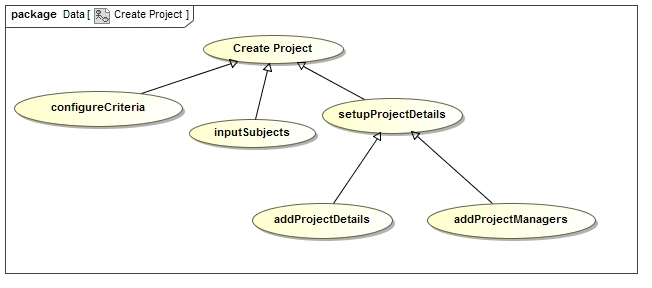
\includegraphics[width=13cm]{./graphics/createProjectUseCase.jpg}
    \rule{0\linewidth}{0.15\linewidth}\par
\begin{enumerate}
\item addProjectDetails\par
Priority: Critical.\par
Pre-condition: Client must be logged in.\par
Post-condition: Client must have a STORM profile.\par
Post-condition: Project skeleton is created in database.\par
\item addProjectManagers\par
Priority: Important.\par
Pre-condition: Client must have a STORM profile.\par
Pre-condition: Manager to be added must have a STORM profile.\par
Pre-condition: Client must have created a STORM project.\par
Post-condition: Manager has permission to collaborate on the project.\par
\item inputSubjects\par
Priority: Critical.\par
Pre-condition: Client must have a STORM profile.\par
Pre-condition: Client must have created a STORM project skeleton.\par
Pre-condition: A .csv file should exist and should be selected.\par
Pre-condition: The .csv should have subjects in it.\par
Post-condition: Project database is updated with a list of subjects.\par
\item configureCriteria\par
Priority: Critical.\par
Pre-condition: Client must have a STORM profile.\par
Pre-condition: Client must be logged into STORM.\par
Pre-condition: Client must have created a STORM project skeleton.\par
Post-condition: Criteria for project is changed.\par
\end{enumerate}
\begin{figure}[h]
    \centering
    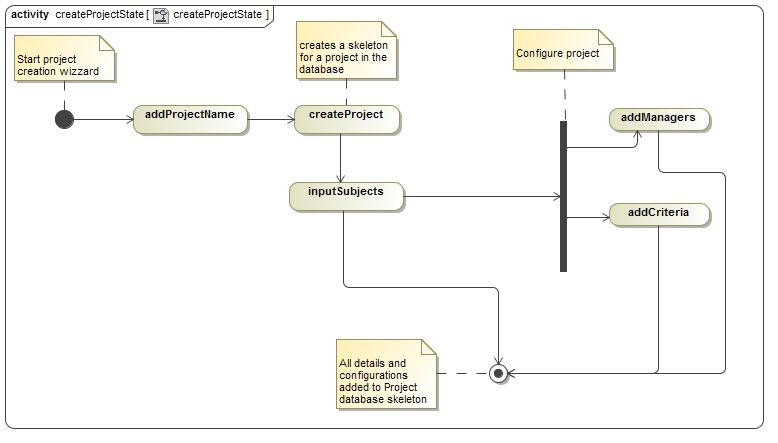
\includegraphics[width=15cm]{./graphics/createProjectState.jpg}
    \caption{createProject sate diagram}
    \label{fig:createProject_state}
\end{figure}